\documentclass{ximera}
\graphicspath{ {./images/} }

\begin{document}
\section*{Answers to Math Placement B-Test Sample Problems}
(1) (a) $x-1$\\
(b) $\frac{2 x^{2}}{x^{2}-1}$\\
(c) $\frac{x}{3 x+1}$\\
(2) $\frac{x^{13}}{y^{16}}$\\
(3) $x+2 y-5=0$\\
(4) $(1,0),(0,2),-2$\\
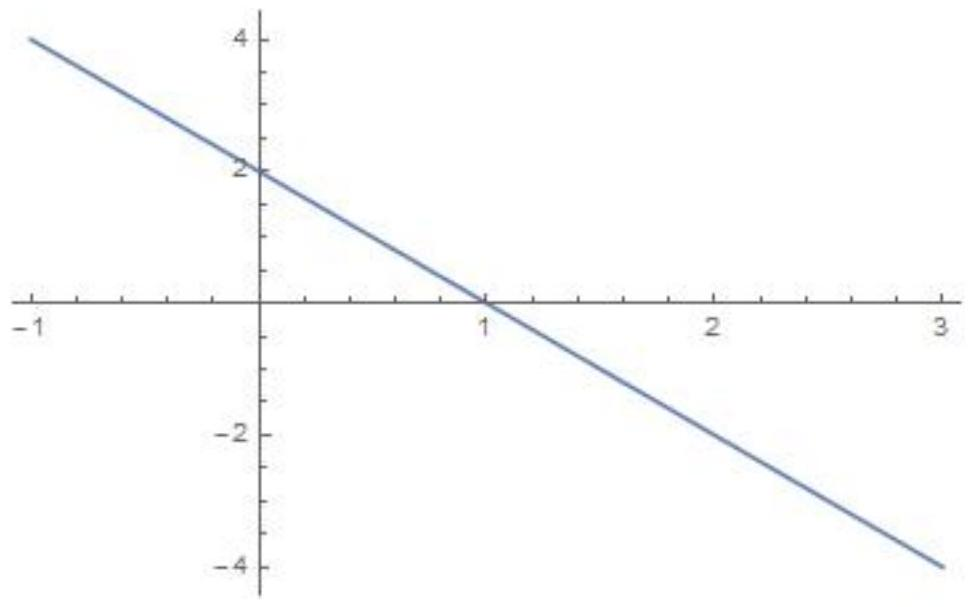
\includegraphics[alt={Graph of a line with negative slope passing through y-intercept 2 and x-intercept 1},width=\textwidth]{line-negative-slope}\\
(5) $x=-5, y=-4$\\
(6) $(2 x+3)(3 x+2)$\\
(7) (a) $x=5,-1$\\
(b) $x=1,-1,3,-3$\\
(c) $x=\frac{1}{2}$\\
(d) $x=\frac{S-2 \pi r^{2}}{8 \pi}$\\
(8)\\
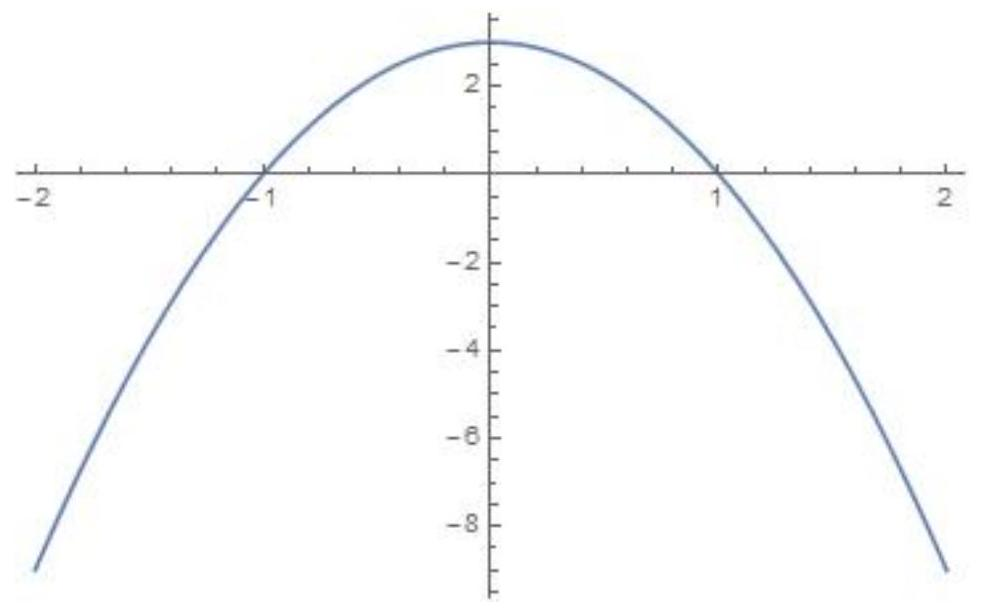
\includegraphics[alt={Graph of a downward-opening parabola with vertex near (0,3) and x-intercepts near negative 1 and 1},width=\textwidth]{downward-parabola}\\
(9) $a=\frac{k b \sqrt{c}}{d^{3}}$\\
(10) $\ell(\overline{\mathrm{BC}})=3 \quad \ell(\overline{\mathrm{AB}})=3 \sqrt{2} \quad \mathrm{~m}(\angle A)=45^{\circ}=\mathrm{m}(\angle B)$\\
(11) $3,7.5,9$\\
(12) 11 inches\\
(13) 18 gallons


\end{document}